\documentclass{standalone}
\usepackage{tikz}
\usetikzlibrary{patterns, positioning}


\begin{document}
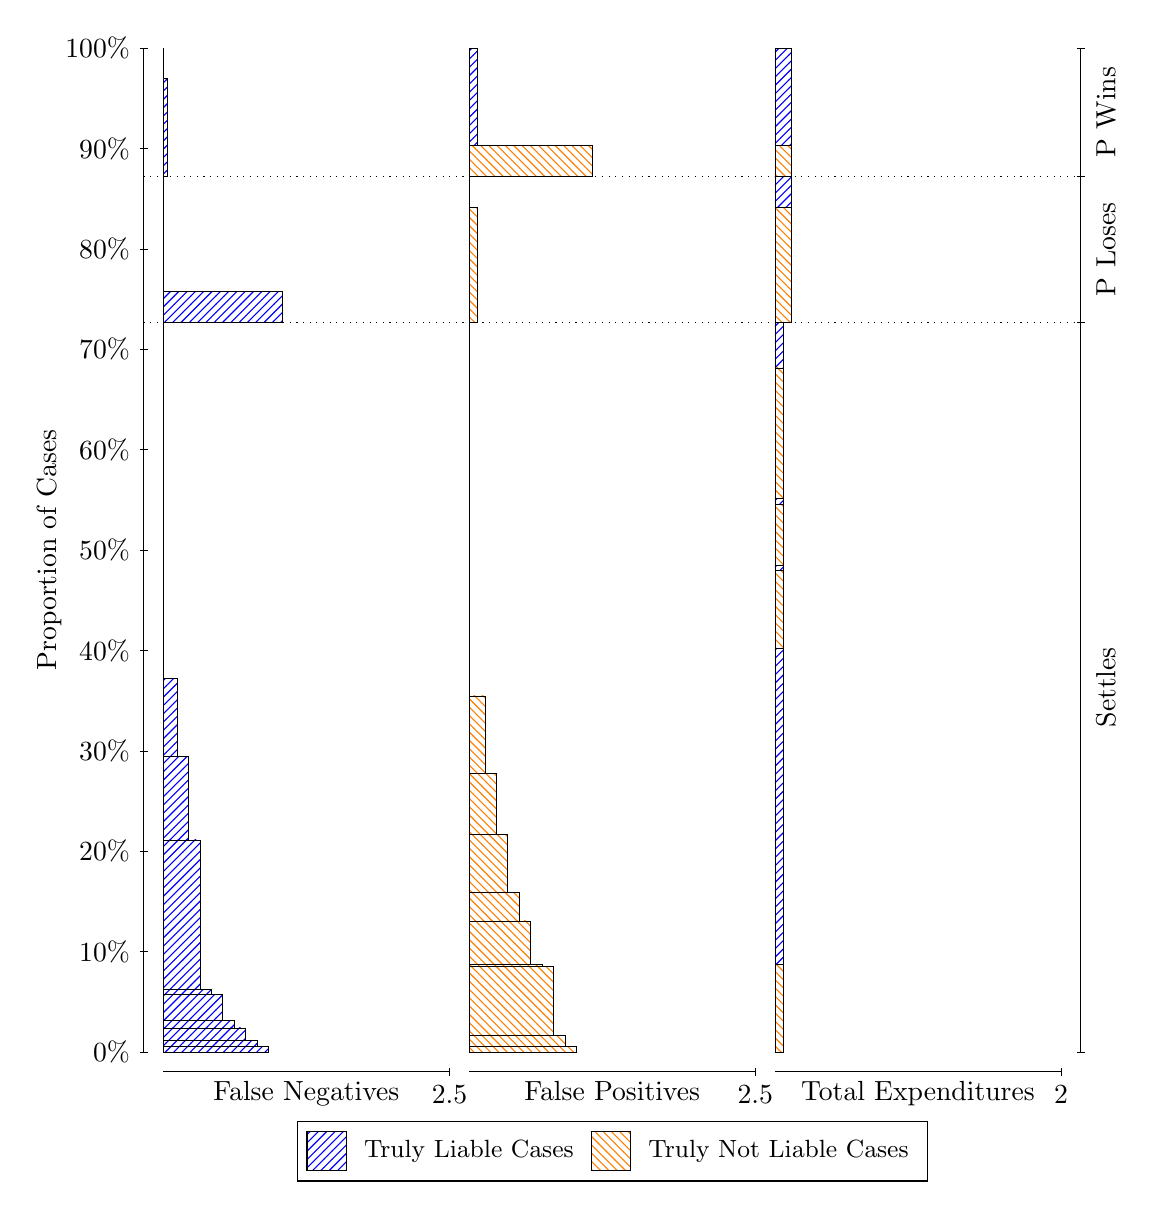
\begin{tikzpicture}
\draw[black, very thin] (1.5,1.75) -- (1.5,14.5);
\node[rotate=90, text=black, anchor=center] at (0.3, 8.125) {Proportion of Cases};
\draw[black, very thin] (1.45,1.75) -- (1.55,1.75);
\node[text=black, anchor=east] at (1.45, 1.75) {0\%};
\draw[black, very thin] (1.45,3.025) -- (1.55,3.025);
\node[text=black, anchor=east] at (1.45, 3.025) {10\%};
\draw[black, very thin] (1.45,4.3) -- (1.55,4.3);
\node[text=black, anchor=east] at (1.45, 4.3) {20\%};
\draw[black, very thin] (1.45,5.575) -- (1.55,5.575);
\node[text=black, anchor=east] at (1.45, 5.575) {30\%};
\draw[black, very thin] (1.45,6.85) -- (1.55,6.85);
\node[text=black, anchor=east] at (1.45, 6.85) {40\%};
\draw[black, very thin] (1.45,8.125) -- (1.55,8.125);
\node[text=black, anchor=east] at (1.45, 8.125) {50\%};
\draw[black, very thin] (1.45,9.4) -- (1.55,9.4);
\node[text=black, anchor=east] at (1.45, 9.4) {60\%};
\draw[black, very thin] (1.45,10.675) -- (1.55,10.675);
\node[text=black, anchor=east] at (1.45, 10.675) {70\%};
\draw[black, very thin] (1.45,11.95) -- (1.55,11.95);
\node[text=black, anchor=east] at (1.45, 11.95) {80\%};
\draw[black, very thin] (1.45,13.225) -- (1.55,13.225);
\node[text=black, anchor=east] at (1.45, 13.225) {90\%};
\draw[black, very thin] (1.45,14.5) -- (1.55,14.5);
\node[text=black, anchor=east] at (1.45, 14.5) {100\%};

\draw[black, very thin] (13.4,1.75) -- (13.4,14.5);
\draw[black, very thin] (13.35,1.75) -- (13.45,1.75);
\node[anchor=west] at (13.35, 1.75) {};
\draw[black, very thin] (13.35,11.016) -- (13.45,11.016);
\node[anchor=west] at (13.35, 11.016) {};
\draw[black, very thin] (13.35,12.87) -- (13.45,12.87);
\node[anchor=west] at (13.35, 12.87) {};
\draw[black, very thin] (13.35,14.5) -- (13.45,14.5);
\node[anchor=west] at (13.35, 14.5) {};

\draw[black, very thin, pattern color=blue, pattern=north east lines] (1.75,1.75) rectangle (3.0852,1.817);
\draw[black, very thin, pattern color=blue, pattern=north east lines] (1.75,1.817) rectangle (2.9399,1.8999);
\draw[black, very thin, pattern color=blue, pattern=north east lines] (1.75,1.8999) rectangle (2.7946,2.0559);
\draw[black, very thin, pattern color=blue, pattern=north east lines] (1.75,2.0559) rectangle (2.6492,2.147);
\draw[black, very thin, pattern color=blue, pattern=north east lines] (1.75,2.147) rectangle (2.5039,2.4773);
\draw[black, very thin, pattern color=blue, pattern=north east lines] (1.75,2.4773) rectangle (2.3586,2.5416);
\draw[black, very thin, pattern color=blue, pattern=north east lines] (1.75,2.5416) rectangle (2.2133,4.4447);
\draw[black, very thin, pattern color=blue, pattern=north east lines] (1.75,4.4447) rectangle (2.0679,5.5065);
\draw[black, very thin, pattern color=blue, pattern=north east lines] (1.75,5.5065) rectangle (1.9226,6.4945);
\draw[black, very thin, pattern color=orange, pattern=north west lines] (1.75,6.4945) rectangle (1.75,11.016);
\draw[black, very thin, pattern color=blue, pattern=north east lines] (1.75,11.016) rectangle (3.2578,11.407);
\draw[black, very thin, pattern color=orange, pattern=north west lines] (1.75,11.407) rectangle (1.75,12.87);
\draw[black, very thin, pattern color=blue, pattern=north east lines] (1.75,12.87) rectangle (1.8045,14.11);
\draw[black, very thin, pattern color=orange, pattern=north west lines] (1.75,14.11) rectangle (1.75,14.5);
\draw[black, very thin, pattern color=orange, pattern=north west lines] (5.6333,1.75) rectangle (6.9958,1.817);
\draw[black, very thin, pattern color=orange, pattern=north west lines] (5.6333,1.817) rectangle (6.8505,1.9619);
\draw[black, very thin, pattern color=orange, pattern=north west lines] (5.6333,1.9619) rectangle (6.7052,2.8322);
\draw[black, very thin, pattern color=orange, pattern=north west lines] (5.6333,2.8322) rectangle (6.5598,2.8613);
\draw[black, very thin, pattern color=orange, pattern=north west lines] (5.6333,2.8613) rectangle (6.4145,3.4144);
\draw[black, very thin, pattern color=orange, pattern=north west lines] (5.6333,3.4144) rectangle (6.2692,3.7743);
\draw[black, very thin, pattern color=orange, pattern=north west lines] (5.6333,3.7743) rectangle (6.1238,4.5175);
\draw[black, very thin, pattern color=orange, pattern=north west lines] (5.6333,4.5175) rectangle (5.9785,5.2838);
\draw[black, very thin, pattern color=orange, pattern=north west lines] (5.6333,5.2838) rectangle (5.8332,6.2719);
\draw[black, very thin, pattern color=blue, pattern=north east lines] (5.6333,6.2719) rectangle (5.6333,11.016);
\draw[black, very thin, pattern color=orange, pattern=north west lines] (5.6333,11.016) rectangle (5.7423,12.479);
\draw[black, very thin, pattern color=blue, pattern=north east lines] (5.6333,12.479) rectangle (5.6333,12.87);
\draw[black, very thin, pattern color=orange, pattern=north west lines] (5.6333,12.87) rectangle (7.1957,13.26);
\draw[black, very thin, pattern color=blue, pattern=north east lines] (5.6333,13.26) rectangle (5.7423,14.5);
\draw[black, very thin, pattern color=orange, pattern=north west lines] (9.5167,1.75) rectangle (9.6189,2.8613);
\draw[black, very thin, pattern color=blue, pattern=north east lines] (9.5167,2.8613) rectangle (9.6189,6.8785);
\draw[black, very thin, pattern color=orange, pattern=north west lines] (9.5167,6.8785) rectangle (9.6189,7.8666);
\draw[black, very thin, pattern color=blue, pattern=north east lines] (9.5167,7.8666) rectangle (9.6189,7.9336);
\draw[black, very thin, pattern color=orange, pattern=north west lines] (9.5167,7.9336) rectangle (9.6189,8.6999);
\draw[black, very thin, pattern color=blue, pattern=north east lines] (9.5167,8.6999) rectangle (9.6189,8.7827);
\draw[black, very thin, pattern color=orange, pattern=north west lines] (9.5167,8.7827) rectangle (9.6189,10.439);
\draw[black, very thin, pattern color=blue, pattern=north east lines] (9.5167,10.439) rectangle (9.6189,11.016);
\draw[black, very thin, pattern color=orange, pattern=north west lines] (9.5167,11.016) rectangle (9.721,12.479);
\draw[black, very thin, pattern color=blue, pattern=north east lines] (9.5167,12.479) rectangle (9.721,12.87);
\draw[black, very thin, pattern color=orange, pattern=north west lines] (9.5167,12.87) rectangle (9.721,13.26);
\draw[black, very thin, pattern color=blue, pattern=north east lines] (9.5167,13.26) rectangle (9.721,14.5);
\draw[black, dotted] (1.5,11.016) -- (13.4,11.016);
\draw[black, dotted] (1.5,12.87) -- (13.4,12.87);
\draw[black, very thin] (1.75,1.5) -- (5.3833,1.5);
\node[text=black, anchor=north] at (3.5667, 1.5) {False Negatives};
\draw[black, very thin] (5.3833,1.45) -- (5.3833,1.55);
\node[text=black, anchor=north] at (5.3833, 1.45) {2.5};

\draw[black, very thin] (5.6333,1.5) -- (9.2667,1.5);
\node[text=black, anchor=north] at (7.45, 1.5) {False Positives};
\draw[black, very thin] (9.2667,1.45) -- (9.2667,1.55);
\node[text=black, anchor=north] at (9.2667, 1.45) {2.5};

\draw[black, very thin] (9.5167,1.5) -- (13.15,1.5);
\node[text=black, anchor=north] at (11.333, 1.5) {Total Expenditures};
\draw[black, very thin] (13.15,1.45) -- (13.15,1.55);
\node[text=black, anchor=north] at (13.15, 1.45) {2};

\node[text=black, centered, rotate=90] at (13.72, 6.3832) {Settles};
\node[text=black, centered, rotate=90] at (13.72, 11.943) {P Loses};
\node[text=black, centered, rotate=90] at (13.72, 13.685) {P Wins};

\draw (7.449999999999999,1.5) node[draw=none] (baseCoordinate) {};
\begin{scope}[align=center]
        \matrix[scale=0.5, draw=black, below=0.5cm of baseCoordinate, nodes={draw}, column sep=0.1cm]{
            \node[rectangle, draw, minimum width=0.5cm, minimum height=0.5cm, pattern color=blue, pattern=north east lines] {}; &
            \node[draw=none, font=\small, text=black] (B) {Truly Liable Cases}; &
            \node[rectangle, draw, minimum width=0.5cm, minimum height=0.5cm, pattern color=orange, pattern=north west lines] {}; &
            \node[draw=none, font=\small, text=black] (B) {Truly Not Liable Cases}; \\
            };
\end{scope}

\end{tikzpicture}
\end{document}